\chapter{Applications}
\label{ch:applications}

\section{Multilingual Translation: 500 Languages to English}

Neural machine translation (NMT)~\cite{bahdanau2014nmtattn,vaswani2017attention} has progressed to reach human performance on select benchmark tasks~\cite{barrault-etal-2019-findings,barrault-etal-2020-findings}. 
However, as MT research has mainly focused on translation between a small number of high resource languages, the unavailability of usable-quality translation models for low resource languages remains an ongoing concern.
Even those commercial translation services attempting to broaden their language coverage has only reached around one hundred languages; this excludes most of the thousands of languages used around the world today.

Freely available corpora of parallel data for many languages are available, though they are hosted at various sites, and are in various forms. A challenge for incorporating more languages into MT models is a lack of easy access to all of these datasets.While standards like ISO 639-3 have been established to bring consistency to the labeling of language resources, these are not yet widely adopted.
In addition, scaling experimentation to several hundred languages on large corpora involves a significant engineering effort.
Simple tasks such as dataset preparation, vocabulary creation, transformation of sentences into sequences, and training data selection becomes formidable at scale due to corpus size and heterogeneity of data sources and file formats.
We have developed tools to precisely address all these challenges, which we demonstrate in this work.
 
Specifically, we offer three tools which can be used either independently or in combination to advance NMT research on a wider set of languages (Section \ref{sec:tools}): firstly, \mtdata, which helps to easily obtain parallel datasets (Section \ref{sec:mtdata}); secondly, \nlcodec, a vocabulary manager and storage layer for transforming sentences to integer sequences, that is efficient and scalable (Section \ref{sec:nlcodec}); and lastly, \rtg, a feature-rich Pytorch-backed NMT toolkit that supports reproducible experiments (Section \ref{sec:rtg}).

We demonstrate the capabilities of our tools by preparing a massive bitext dataset with more than 9 billion tokens per side, and training a single multilingual NMT model capable of translating 500 source languages to English (Section \ref{sec:500-eng}).
We show that the multilingual model is usable either as a service for translating several hundred languages to English (Section \ref{sec:value.off-shelf-mt}), or as a parent model in a transfer learning setting for improving translation of low resource languages (Section \ref{sec:value.transfer-learning}). 
%pretrained multilingual embeddings (Section \ref{sec:value.embeddings}),


\section{Tools}
\label{sec:tools}
 Our tools are organized into the following sections:

\begin{comment}
Specifically, \textsc{MTData} (Section \ref{sec:mtdata}) is useful for preparing training data for hundreds of languages, 
\textsc{NLCodec} (section \ref{sec:nlcodec}) is useful for efficiently proprocessing, storing, and accessing the training data,
and \textsc{RTG} (section \ref{sec:rtg}) NMT toolkit for training an MT model. 
In addition, all these tools are built with reproducibility and usability in mind. 
These tools have been made publicly available, with permissive open source licenses.
We hope these tools help advance MT efforts beyond the top few high resource languages. 
\end{comment}

\subsection{\textsc{MTData}}
\label{sec:mtdata}
\textsc{MTData} addresses an important yet often overlooked challenge -- dataset preparation. 
By assigning an ID for datasets, we establish a clear way of communicating the exact datasets used for MT experiments, which helps in reproducing the experimental setup.
By offering a unified interface to datasets from many heterogeneous sources, \mtdata\ hides mundane tasks such as locating URLs, downloading, decompression, parsing, and sanity checking. Some noteworthy features are:
\begin{itemize}[noitemsep,topsep=0pt,leftmargin=4mm]
\item \textit{Indexer}: a large index of publicly available parallel datasets.
\item \textit{Normalizer:} maps language names to ISO-639-3 codes which has representation space for 7800+ languages.\footnote{\url{https://iso639-3.sil.org}}
\item \textit{Parsers:} parses heterogeneous data formats for parallel datasets, and produces a simple plain text file by merging all the selected datasets.
\item \textit{Extensible:} new datasets and parsers can be easily added.
\item \textit{Local Cache}: reduces network transfers by maintaining a local cache, which is shared between experiments.
\item \textit{Sanity Checker}: performs basic sanity checks such as segment count matching and empty segment removal. When error states are detected, stops the setup with useful error messages.
\item \textit{Reproducible:} stores a signature file that can be used to recreate the dataset at a later time.
\item \textit{Courtesy:} shows the original \BibTeX\ citation attributed to datasets.
\item \textit{Easy Setup:} \texttt{pip install mtdata}
\item \textit{Open-source:} \\ \url{https://github.com/thammegowda/mtdata}
\end{itemize}

Listing \ref{lst:mtdata-eg} shows an example for listing and getting datasets for German-English.
\begin{listing}
\begin{minted}[baselinestretch=1, fontsize=\footnotesize, frame=lines, framesep=2mm,]{bash}
# List all the available datasets for deu-eng
$ mtdata list -l deu-eng
# Get the selected training & held-out sets
$ mtdata get -l deu-eng --merge\
 -tr wmt13_europarl_v7 wmt13_commoncrawl\ 
    wmt18_news_commentary_v13\
 -ts newstest201{8,9}_deen -o data
\end{minted}
\caption{\mtdata\ examples for listing and downloading German-English datasets.
The \texttt{--merge} flag results in merging all of the training datasets specified by \texttt{-tr} argument into a single file. }
\label{lst:mtdata-eg}
\end{listing}
 In Section~\ref{sec:datasets}, we use \mtdata\footnote{At the time of writing, v0.2.8} to obtain thousands of publicly available datasets for a large many-to-English translation experiment.

\subsection{\nlcodec}
\label{sec:nlcodec}
\nlcodec\ is a vocabulary manager with encoding-decoding schemes to transform natural language sentences to and from integer sequences.\\
\textbf{Features:}
\begin{itemize}[noitemsep,topsep=0pt,leftmargin=4mm]
\item \textit{Versatile:} Supports commonly used vocabulary schemes such as characters, words, and byte-pair-encoding (BPE) subwords~\cite{sennrich-etal-2016-bpe}.
\item \textit{Scalable:} Apache Spark\footnote{\url{https://spark.apache.org/}}\cite{zaharia2016spark} backend can be optionally used to create vocabulary from massive datasets.
\item \textit{Easy Setup:} \texttt{pip install nlcodec} 
\item \textit{Open-source:}\\ \url{https://github.com/isi-nlp/nlcodec/}
\end{itemize}

When the training datasets are too big to be kept in the primary random access memory (RAM), the use of secondary storage is inevitable.
The training processes requiring random examples lead to random access from a secondary storage device.
Even though the latest advancements in secondary storage technology such as solid-state drive (SSD) have faster serial reads and writes, their random access speeds are significantly lower than that of RAM. 
%In addition, since sentences are of variable lengths, use of fixed sized tensors are not feasible. 
To address these problems, we include an efficient storage and retrieval layer, \nldb, which has the following features:
\begin{itemize}[noitemsep,topsep=0pt,leftmargin=4mm]
  \item \textit{Memory efficient} by adapting datatypes based on vocabulary size. For instance, encoding with vocabulary size less than 256 (such as characters) can be efficiently represented using 1-byte unsigned integers. Vocabularies with fewer than 65,536 types, such as might be generated when using subword models \cite{sennrich-etal-2016-bpe} require only 2-byte unsigned integers, and 4-byte unsigned integers are sufficient for vocabularies up to 4 billion types. 
As the default implementation of Python, CPython, uses 28 bytes for all integers, we accomplish this using NumPy~\cite{harris2020numpy}. This optimization makes it possible to hold a large chunk of training data in smaller RAM, enabling a fast random access.
  \item \textit{Parallelizable:} Offers a multi-part database by horizontal sharding that supports parallel writes (e.g., Apache Spark) and parallel reads (e.g., distributed training).
%  \item \textit{I/O efficient:} Reads and writes large blocks at once instead of multiple smaller chunks, thus taking advantage of faster serial reads and write speeds.
  \item Supports commonly used batching mechanisms such as random batches with approximately-equal-length sequences.
\end{itemize}

\nldb\ has a minimal footprint and is part of the \nlcodec\ package.
In Section~\ref{sec:500-eng}, we take advantage of the scalability and efficiency aspects of \nlcodec\ and \nldb\ to process a large parallel dataset with 9 billion tokens on each side.


\subsection{\rtg}
\label{sec:rtg}
Reader translator generator (\rtg) is a neural machine translation (NMT) toolkit based on Pytorch~\cite{NEURIPS2019_Pytorch}. 
Notable features of \rtg\ are:
\begin{itemize}[noitemsep,topsep=0pt,leftmargin=4mm]
\item \textit{Reproducible:} All the required parameters of an experiment are included in a single YAML configuration file, which can be easily stored in a version control system such as \texttt{git} or shared with collaborators.
\item Implements Transformer~\cite{vaswani2017attention}, and recurrent neural networks (RNN) with cross-attention models ~\cite{bahdanau2014nmtattn,luong2015effectiveAttn}.
%cho2014GRU,hochreiter1997LSTM
\item Supports distributed training on multi-node multi-GPUs, gradient accumulation, and Float16 operations.
\item Integrated Tensorboard helps in visualizing training and validation losses. 
% shows training speed, estimated finish time on \texttt{tqdm} progress-bar. 
\item Supports weight sharing~\cite{press-wolf-2017-embeddings}, parent-child transfer~\cite{zoph-etal-2016-transfer}, beam decoding with length normalization~\cite{wu-etal-2016-GNMT}, early stopping, and checkpoint averaging. 
%, and transfer learning with selective layer weight freezing. 
\item Flexible vocabulary options with \nlcodec\ and \sentpiece~\cite{kudo-richardson-2018-sentencepiece} which can be either shared or separated between source and target languages.
\item \textit{Easy setup:} \texttt{pip install rtg}
%\item A CLI for running end-to-end experiments based on a YAML config file (\texttt{rtg-pipe}); also supports experiment forking and export (\texttt{rtg-fork}, \texttt{rtg-export}).
%\item In addition to CLI interface for translation generation (\texttt{rtg-decode}), web and REST interfaces are also supported (\texttt{rtg-serve}).
\item \textit{Open-source:} \url{https://isi-nlp.github.io/rtg/}
\end{itemize}

\begin{comment}
% [
%frame=lines,
%framesep=2mm,
% baselinestretch=1.1,
% fontsize=\footnotesize,
%linenos
%]{bash}
\begin{listing}[ht]
\scriptsize
%\tiny
\inputminted{yaml}{sample-conf.yml}
\caption{An example \textit{conf.yml} file from an RTG experiment.}
\end{listing}


\begin{table}[]
    \centering
    \footnotesize
    \begin{tabular}{l  l| r r}
        NMT & BPE Impl  & NewsTest18 & NewsTest19 \\ \hline \hline
        \rtg & \nlcodec\   & 32.6   & 29.0 \\
        \rtg & \scriptsize{\sentpiece\ }& 32.3 & 28.7 \\
        FairSeq & subword-nmt & & \\
        T2T &  (built-in) & &
    \end{tabular}
    \caption{Transformer-base model is trained on the datasets shown in Listing~\ref{lst:mtdata-eg} for 200K optimizer updates having a batch size of 4200 tokens. All models use shared 8000 BPE subwords as vocabulary. The BLEU scores are from \sacrebleu\ \texttt{BLEU+c.mixed+l.de-en+\#.1+s.exp+
    t.wmt1\{8,9\}+tok.13a+v.1.4.13}.  }
    \label{tab:my_label}
\end{table}

\end{comment}



\section{Many-to-English Multilingual NMT}
\label{sec:500-eng}
In this section, we demonstrate the use of our tools by creating a massively multilingual NMT model from publicly available datasets. 

\subsection{Dataset}
\label{sec:datasets}
We use \mtdata\ to download datasets from various sources, given in Table~\ref{tab:data-sources}. 
To minimize data imbalance, we select only a subset of the datasets available for high resource languages, and select all available datasets for low resource languages. The selection is aimed to increase the diversity of data domains and quality of alignments. 

 \begin{table}[ht]
 \centering
 %\footnotesize
 \begin{tabular}{p{0.3\linewidth} p{0.7\linewidth}}
  Dataset   & Reference \\ \hline\hline
 Europarl    & \citet{koehn2005europarl} \\
 KFTT Ja-En & \citet{neubig11kftt}  \\ 
 Indian6     & \citet{post-etal-2012-constructing}   \\ 
 OPUS        & \citet{tiedemann-2012-parallel}  \\
 UNPCv1     & \citet{ziemski-etal-2016-unpc}   \\
 Tilde MODEL & \citet{rozis-skadins-2017-tilde}  \\
 TEDTalks    & \citet{qi-etal-2018-pretrainemb}  \\ 
 IITB Hi-En & \citet{kunchukuttan-etal-2018-iit} \\
 Paracrawl   & \citet{espla-etal-2019-paracrawl} \\
 WikiMatrix & \citet{schwenk-etal-2019-wikimatrixv1} \\
 JW300       & \citet{agic-vulic-2019-jw300}  \\
 PMIndia & \citet{haddow2020pmindia}  \\
 OPUS100    & \citet{zhang-etal-2020-multiling-nmt} \\
 WMT [13-20] & \citet{bojar-etal-2013-findings, bojar-etal-2014-findings, bojar-etal-2015-findings, bojar-etal-2016-findings, bojar-etal-2017-findings, bojar-etal-2018-findings, barrault-etal-2019-findings, barrault-etal-2020-findings} \\

 \end{tabular}
 \caption{Various sources of MT datasets.}
 \label{tab:data-sources}
\end{table}

%\begin{figure*}[ht]
\begin{sidewaysfigure}
\centering
    %trim={5mm 4mm 5mm 5mm},clip
    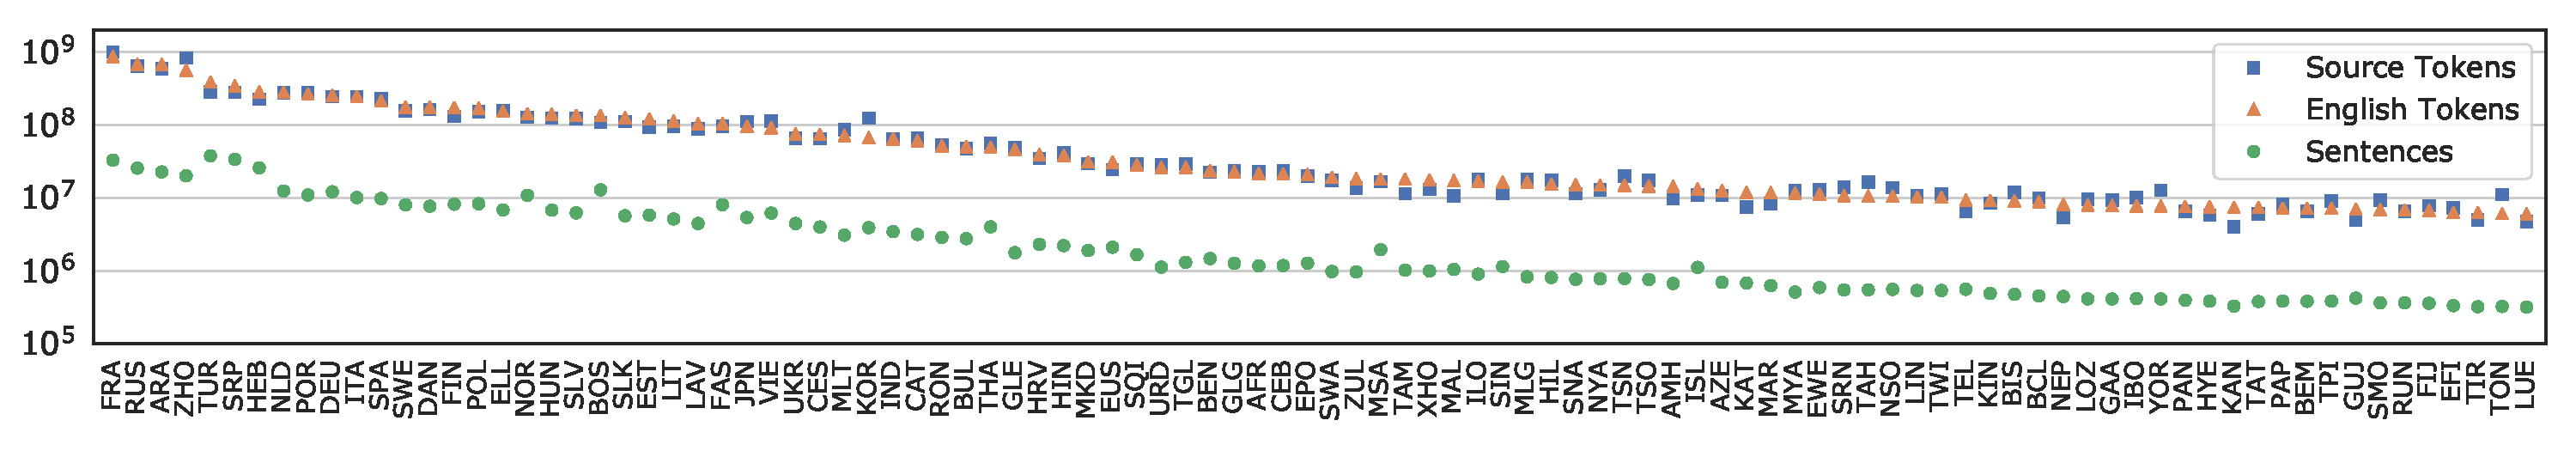
\includegraphics[height=0.14\vsize,trim={5mm 4mm 5mm 5mm},clip]{manyeng/lang-stats-1-100.pdf}
    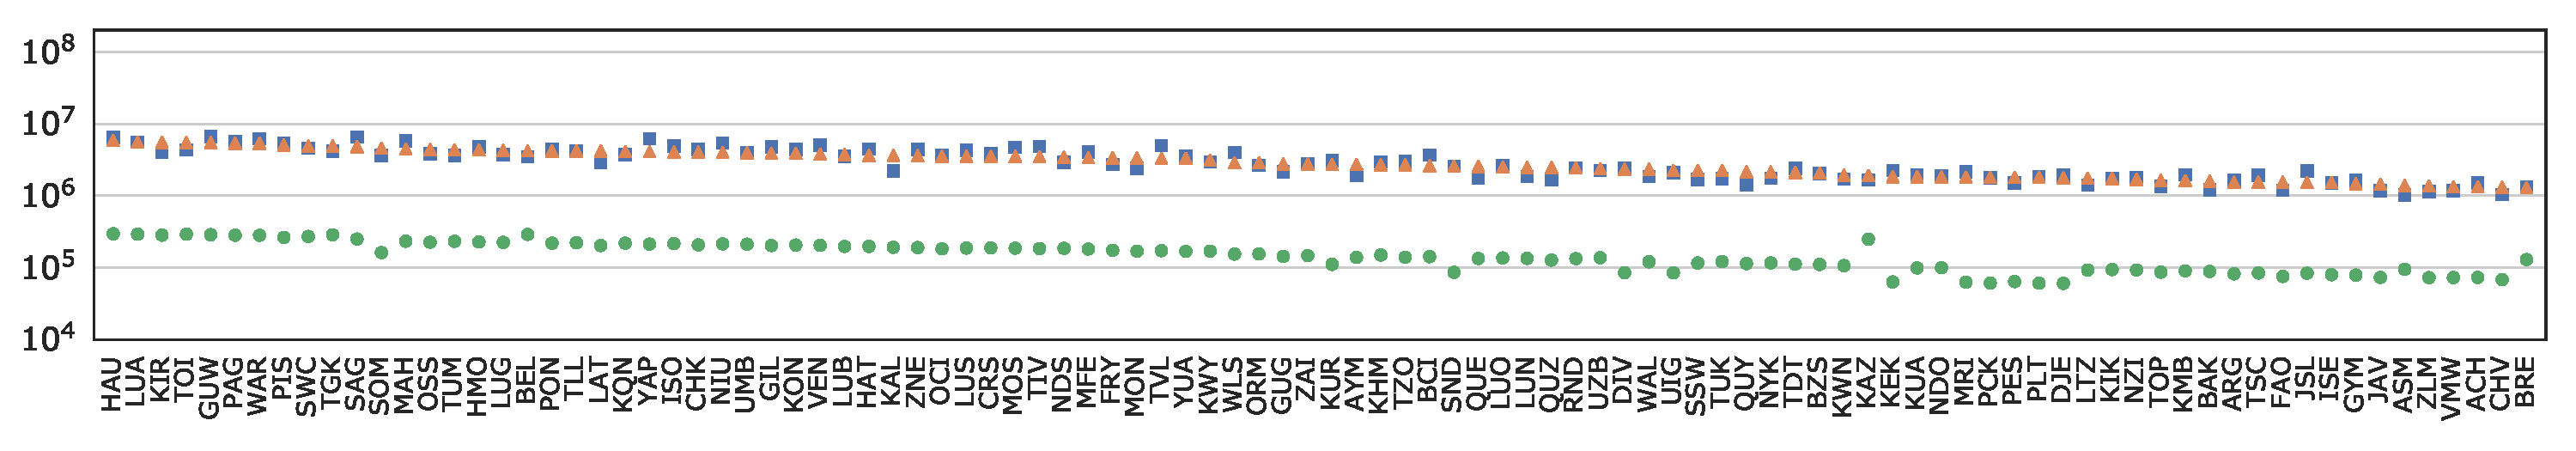
\includegraphics[height=0.14\vsize,trim={5mm 4mm 5mm 5mm},clip]{manyeng/lang-stats-101-200.pdf}
    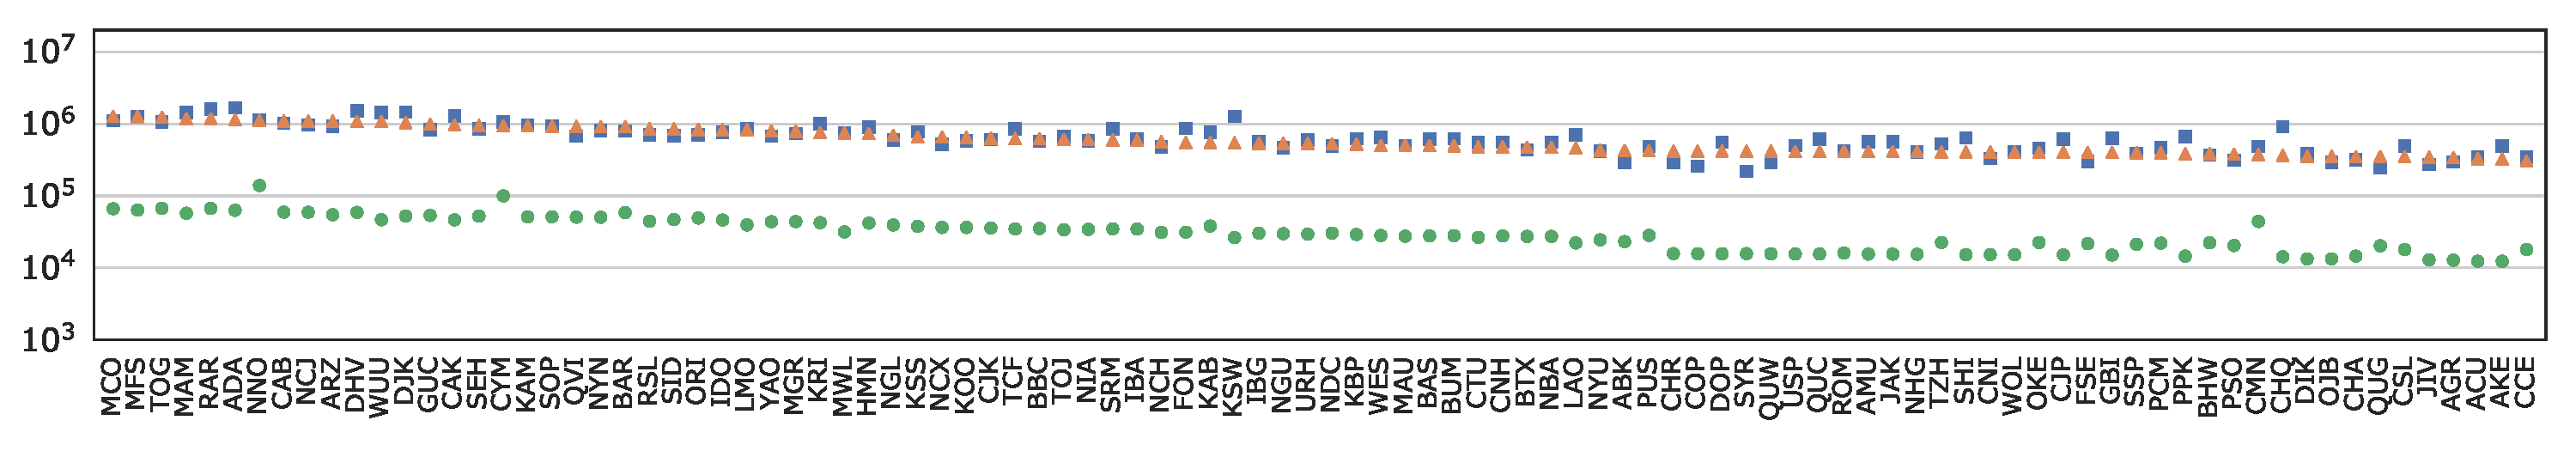
\includegraphics[height=0.14\vsize,trim={5mm 4mm 5mm 5mm},clip]{manyeng/lang-stats-201-300.pdf}
    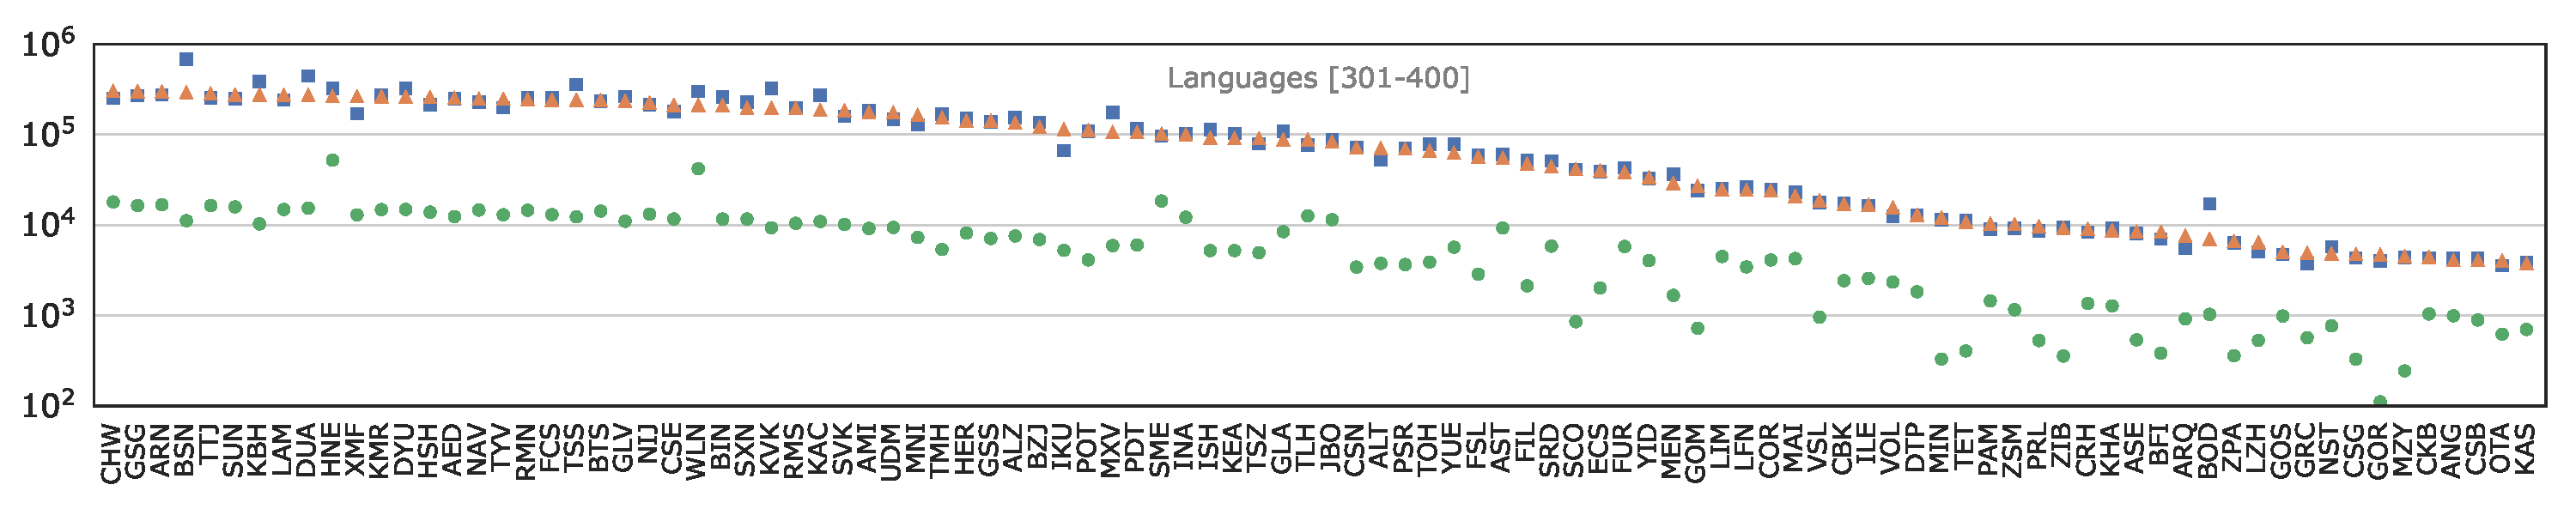
\includegraphics[height=0.14\vsize,trim={5mm 4mm 5mm 5mm},clip]{manyeng/lang-stats-301-400.pdf}
    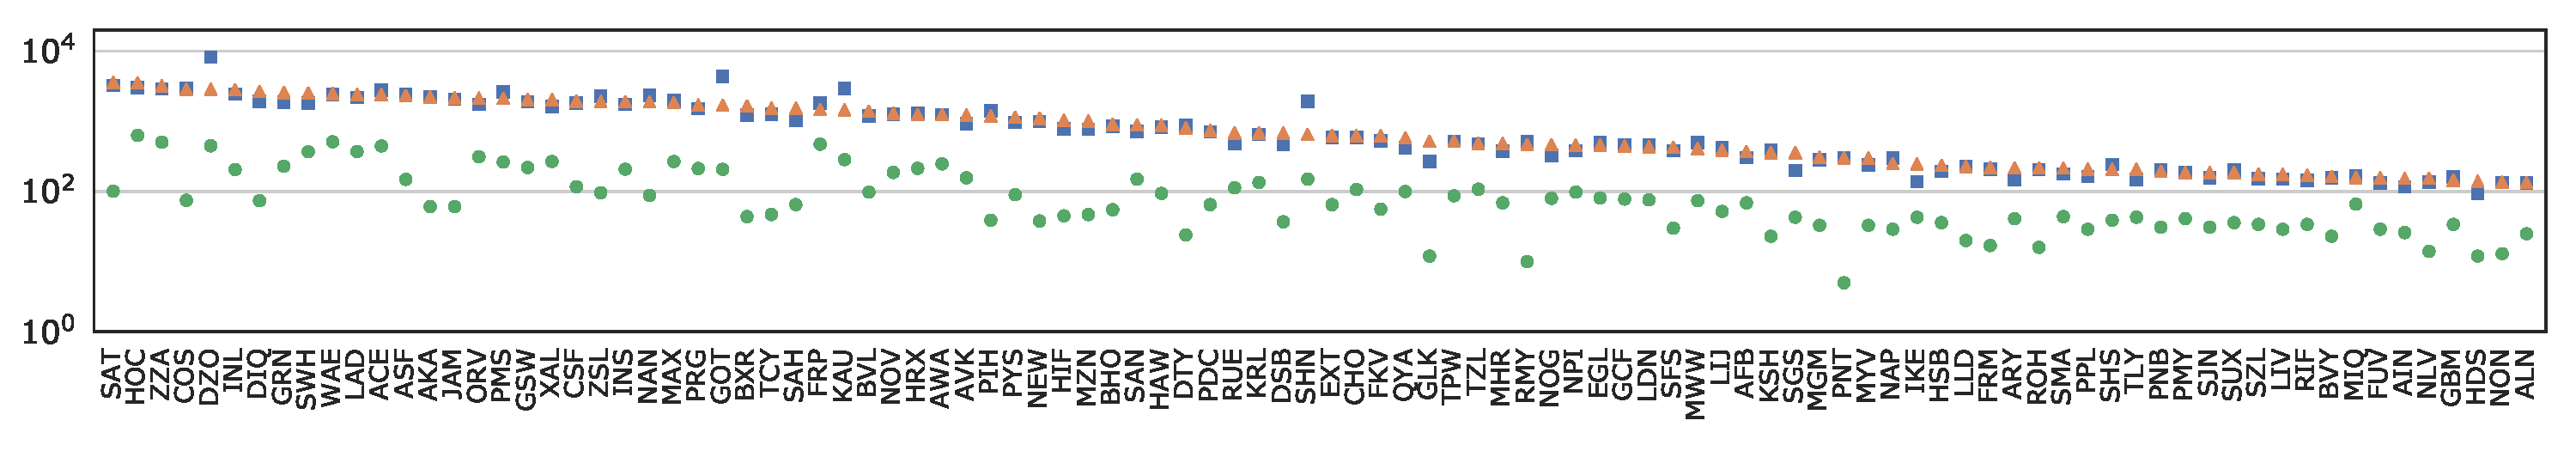
\includegraphics[height=0.14\vsize,trim={5mm 4mm 5mm 5mm},clip]{manyeng/lang-stats-401-500.pdf}     
    \caption{\centering Training data statistics for 500 languages, sorted as descending order of English token count,  obtained after de-duplication and filtering (see Section~\ref{sec:datasets}). The full name for these ISO 639-3 codes can be looked up using \mtdata, e.g. \texttt{mtdata-iso eng}. }
       \label{fig:train-data-stats}
\end{sidewaysfigure}
%\end{figure*}


\textbf{Cleaning:}
 We use \textsc{SacreMoses}\footnote{\url{https://github.com/isi-nlp/sacremoses} a fork of \url{https://github.com/alvations/sacremoses} with improvements to tokenization for many low resource languages.} to normalize Unicode punctuations and digits, followed by word tokenization. 
We remove records that are duplicates, have abnormal source-to-target length ratios, have many non-ASCII characters on the English side, have a URL, or which overlap exactly, either on the source or target side, with any sentences in held out sets.
As preprocessing is compute-intensive, we parallelize using Apache Spark.
The cleaning and tokenization results in a corpus of 474 million sentences and 9 billion tokens on the source and English sides each. The token and sentence count for each language are provided in Figure~\ref{fig:train-data-stats}.
Both the processed and raw datasets are available at \url{http://rtg.isi.edu/many-eng/data/v1/}.\footnote{A copy is at \url{https://opus.nlpl.eu/MT560.php}}

\subsection{Many-to-English Multilingual Model}
\label{sec:500eng-model}
We use \rtg\ to train Transformer NMT \cite{vaswani2017attention} with a few modifications.
Firstly, instead of a shared BPE vocabulary for both source and target, we use two separate BPE vocabularies. 
Since the source side has 500 languages but the target side has English only, we use a large source vocabulary and a relatively smaller target vocabulary.
A larger target vocabulary leads to higher time and memory complexity, whereas a large source vocabulary increases only the memory complexity but not the time complexity.
We train several models, ranging from the standard 6 layers, 512-dimensional Transformers to larger ones with more parameters. Since the dataset is massive, a larger model trained on big mini-batches yields the best results. Our best performing model is a 768 dimensional model with 12 attention heads, 9 encoder layers, 6 decoder layers, feed-forward dimension of 2048, dropout and label smoothing at 0.1, using $512,000$ and $64,000$ BPE types as source and target vocabularies, respectively. The decoder's input and output embeddings are shared.
Since some of the English sentences are replicated to align with many sentences from different languages (e.g. the Bible corpus), BPE merges are learned from the deduplicated sentences using \nlcodec.
Our best performing model is trained with an effective batch size of about 720,000 tokens per optimizer step. Such big batches are achieved by using mixed-precision distributed training on 8 NVIDIA A100 GPUs with gradient accumulation of 5 mini-batches, each having a maximum of 18,000 tokens. We use the Adam optimizer~\cite{kingma2015adam} with 8000 warm-up steps followed by a decaying learning rate, similar to \citet{vaswani2017attention}. 
We stop training after five days and six hours when a total of 200K updates are made by the optimizer; validation loss is still decreasing at this point. 
To assess the translation quality of our model, we report BLEU~\cite{papineni-etal-2002-bleu,post-2018-sacrebleu}\footnote{All our BLEU scores are obtained from \sacrebleu\ \texttt{BLEU+c.mixed+\#.1+s.exp+tok.13a+v.1.4.13}.} on a subset of languages for which known test sets are available, as given in Figure~\ref{fig:test-bleu}, along with a comparison to \citet{zhang-etal-2020-multiling-nmt}'s best model.\footnote{
%a multilingual 24-layered 512-dimensional Transformer model having Merged Attention, Language-aware Layer Normalization and Linear Transformation, and trained including random online backtranslation.
Scores are obtained from \url{https://github.com/bzhangGo/zero/tree/master/docs/multilingual_laln_lalt}; accessed: 2021/03/30}

\begin{figure*}[ht]
    \centering
    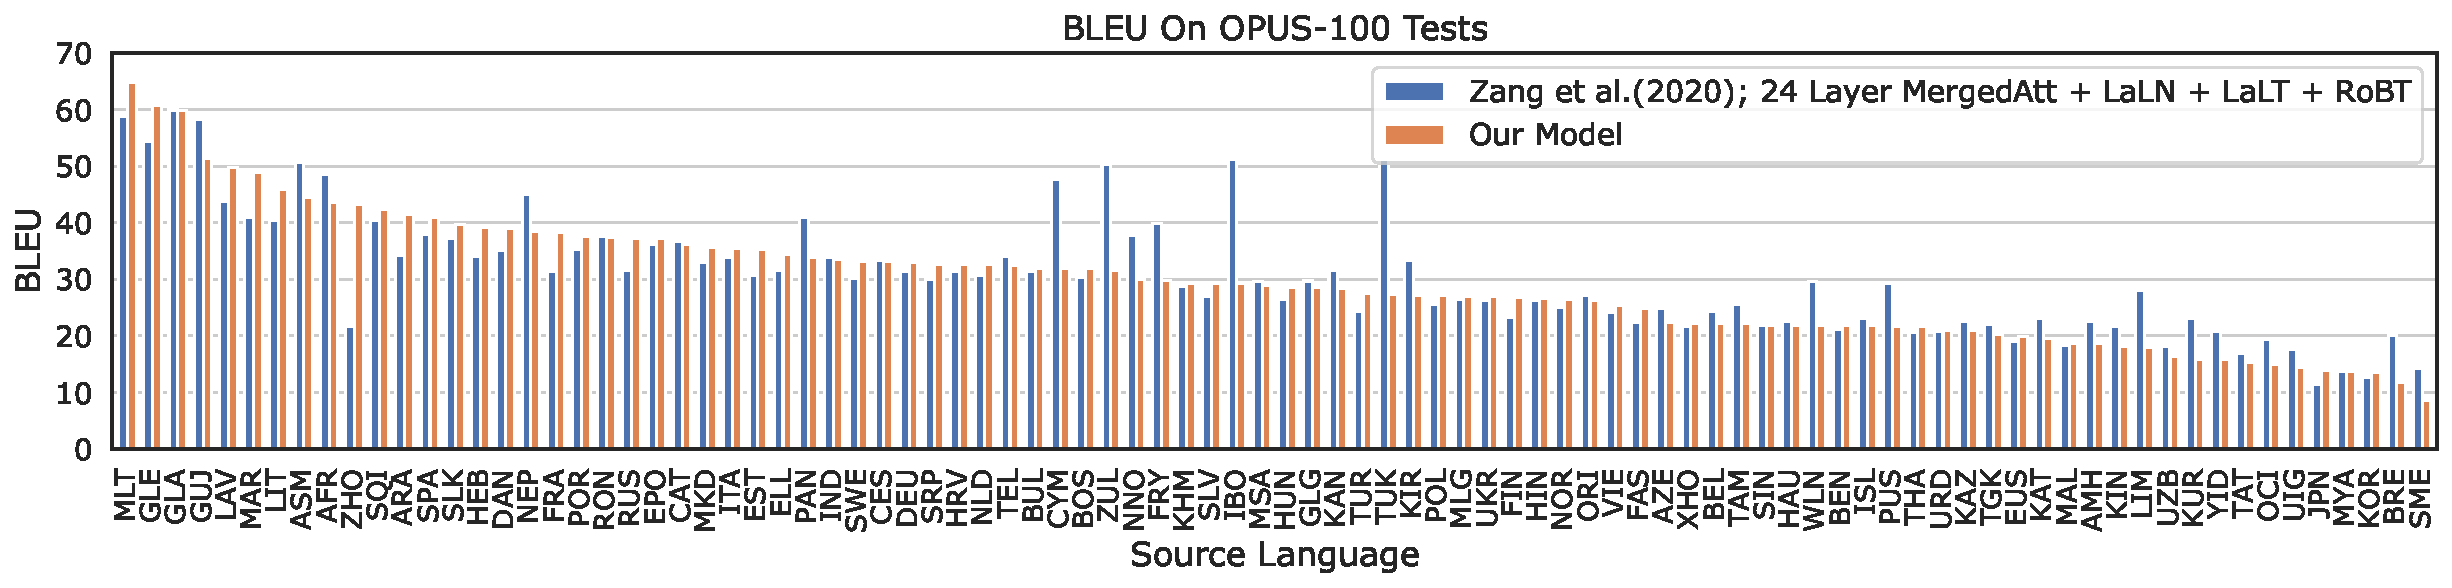
\includegraphics[width=\textwidth]{manyeng/BLEU-opus100.pdf}
    \caption[Caption for LOF]{Many-to-English BLEU on OPUS-100 tests~\cite{zhang-etal-2020-multiling-nmt}. 
    Despite having four times more languages on the source side, our model scores competitive BLEU on most languages with the strongest system of \citet{zhang-etal-2020-multiling-nmt}. The tests where our model scores lower BLEU have shorter source sentences (mean length of about three tokens).}
    \label{fig:test-bleu}
\end{figure*}
%All BLEU scores are mixed-cased and are obtained using the default settings of \sacrebleu.
% https://github.com/bzhangGo/zero/tree/master/docs/multilingual_laln_lalt

\begin{comment}
\begin{subfigure}[t]{0.68\textwidth}
        \centering
        \includegraphics[width=\linewidth]{manyeng/BLEU-nttalksv1.pdf}
        %\caption{Lorem ipsum}
    \end{subfigure}%
    ~ 
    \begin{subfigure}[t]{0.31\textwidth}
        \centering
        \includegraphics[width=\linewidth,trim={7mm 0mm 0mm 0mm},clip]{img/BLEU-wmt-etc.pdf}
        %\caption{Lorem ipsum}
    \end{subfigure}
     TED Talks~\cite{qi-etal-2018-pretrainemb}, WMT~\cite{barrault-etal-2019-findings}, UNv1~\cite{ziemski-etal-2016-unpc}, and Indian-6~\cite{post-etal-2012-constructing}.
\end{comment}



\section{Applications}
\label{sec:value}
The model we trained as a demonstration for our tools is useful on its own, as described in the following sections. 

\subsection{Readily Usable Translation Service}
\label{sec:value.off-shelf-mt}
Our pretrained NMT model is readily usable as a service capable of translating several hundred source languages to English.
By design, source language identification is not necessary.
Figure~\ref{fig:test-bleu} shows that the model scores more than 20 BLEU, which maybe be a useful quality for certain downstream applications involving web and social media content analysis.
Apache Tika \cite{mattmann2011tika}, a content detection and analysis toolkit capable of parsing thousands of file formats, has an option for translating any document into English using our multilingual NMT model.\footnote{\url{https://cwiki.apache.org/confluence/display/TIKA/NMT-RTG}} Our model has been packaged and published to DockerHub\footnote{\url{https://hub.docker.com/}}, which can be obtained by the following command:
\begin{minted}[
%frame=lines,
%framesep=2mm,
baselinestretch=1.1,
fontsize=\small,
%linenos
]{bash}
IMAGE=tgowda/rtg-model:500toEng-v1
docker run --rm -i -p 6060:6060 $IMAGE 
# For GPU support: --gpus '"device=0"' 
\end{minted}

The above command starts a docker image with HTTP server having a web interface, as can be seen in Figure~\ref{fig:rtg-webui}, and a REST API.
An example interaction with the REST API is as follows: 
\begin{figure}[ht]
    \centering
    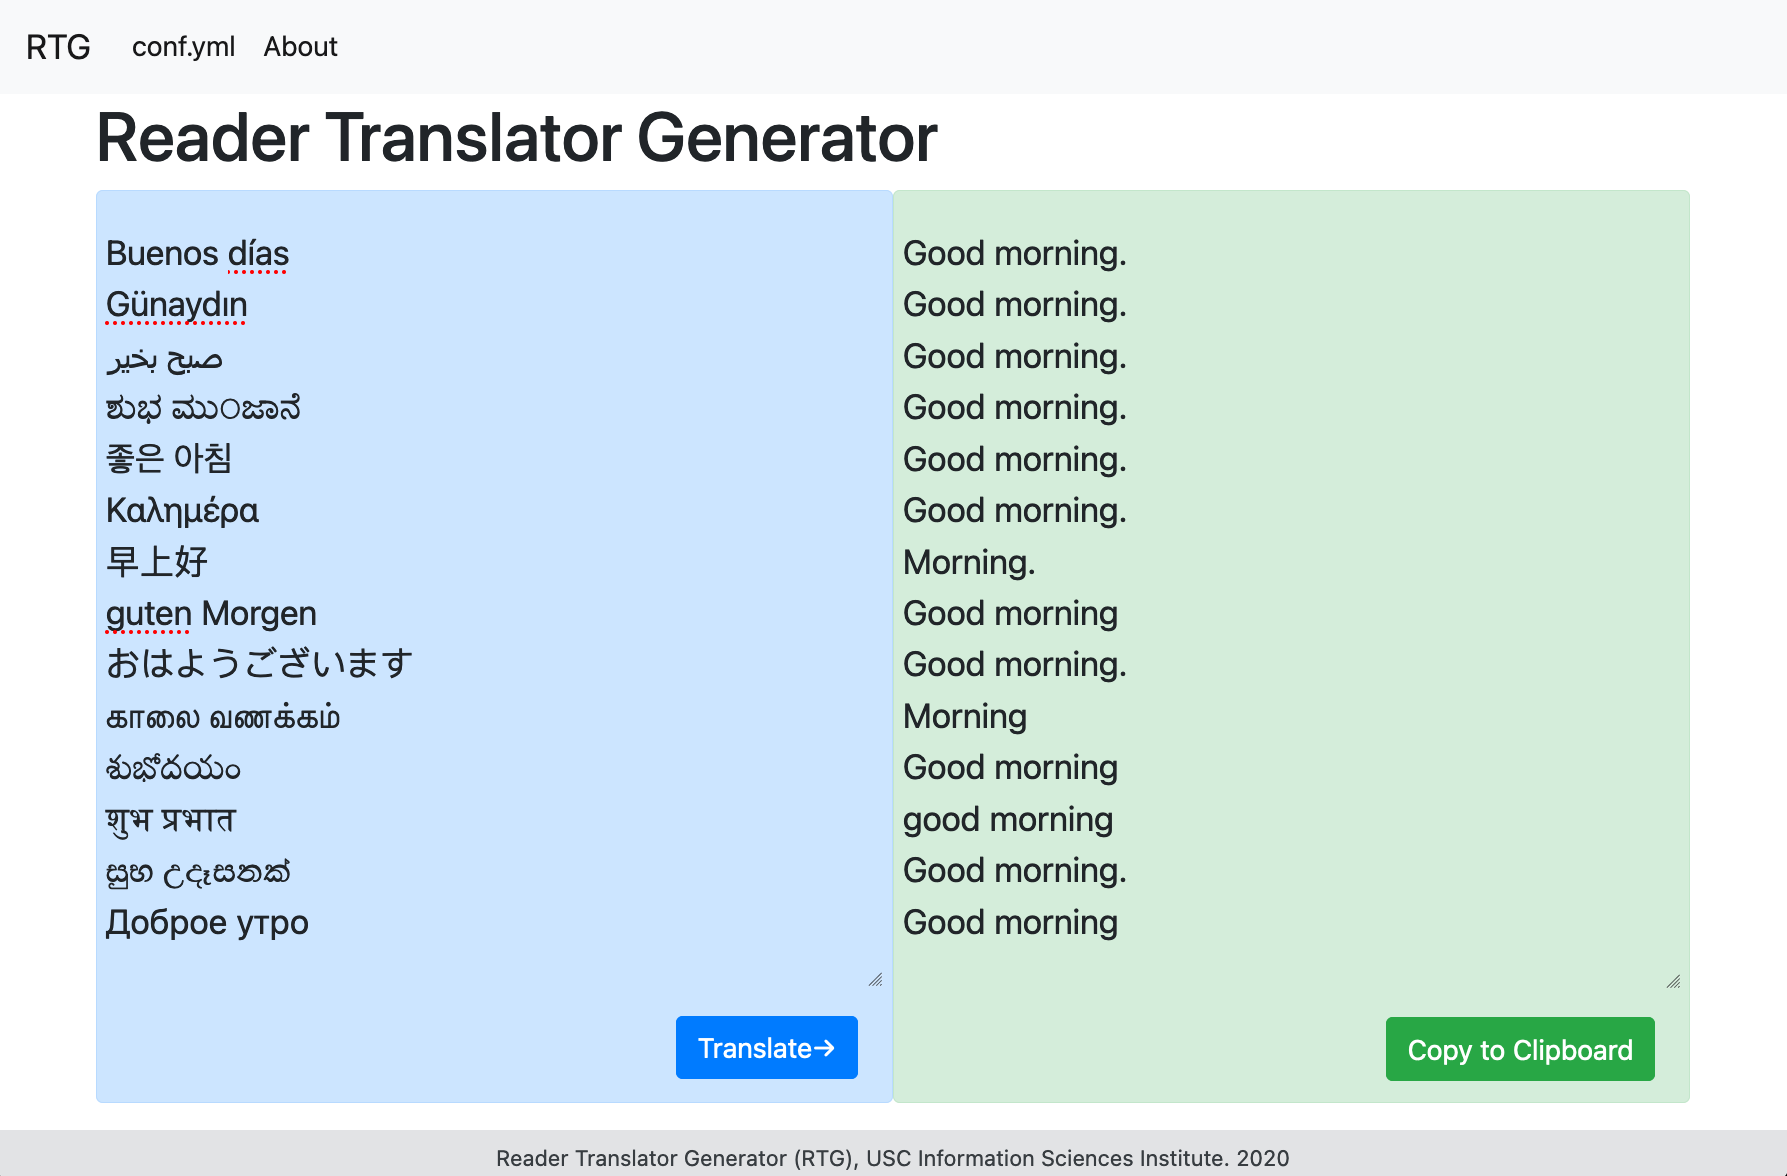
\includegraphics[width=0.6\linewidth,trim=20 60 100 15,clip]{manyeng/rtg-webui.png}
    \caption{RTG Web Interface}
    \label{fig:rtg-webui}
\end{figure}

\begin{minted}[baselinestretch=1.1, fontsize=\small]{bash}
curl --data "source=Comment allez-vous?"\
    --data "source=Bonne journée"\
    http://localhost:6060/translate
\end{minted}
\begin{minted}[baselinestretch=1.1, fontsize=\small]{json}
 {
  "source": [ "Comment allez-vous?",
        "Bonne journée" ],
  "translation": [ "How are you?", 
         "Have a nice day" ]
}
\end{minted}


\subsection{Parent Model for Low Resource MT}
\label{sec:value.transfer-learning}
%WMT 20 has two low resource languages: IU and KM http://statmt.org/wmt20/translation-task.html 
%Uyghur from Lorelei?  Pashto  from Material?
 Fine tuning is a useful transfer learning technique for improving the translation of low resource languages ~\cite{zoph-etal-2016-transfer,neubig-hu-2018-rapid,gheini2019universal}. 
For instance, consider Breton-English (BRE-ENG) and Northern Sami-English (SME-ENG), two of the low resource settings for which our model has relatively poor BLEU (see Figure~\ref{fig:test-bleu}). 
To show the utility of fine tuning with our model, we train a strong baseline Transformer model, one for each language, from scratch using OPUS-100 training data~\cite{zhang-etal-2020-multiling-nmt}, and finetune our multilingual model on the same dataset as the baselines. We shrink the parent model vocabulary and embeddings to the child model dataset, and train all models on NVIDIA P100 GPUs until convergence.\footnote{More info: \url{https://github.com/thammegowda/006-many-to-eng/tree/master/lowres-xfer}}
 Table~\ref{tab:transfer-lowres}, which shows BLEU on the OPUS-100 test set for the two low resource languages indicates that our multilingual NMT parent model can be further improved with finetuning on limited training data. The finetuned model is significantly better than baseline model.

\begin{table}[ht]
    \centering
    %\footnotesize
    \begin{tabular}{l  r r}
        Model     & BRE-ENG & SME-ENG \\ \hline\hline
        Baseline  & 12.7  &  10.7  \\
        Parent    & 11.8  &  8.6  \\
        \textit{Finetuned} & \textbf{22.8}  & \textbf{19.1}  \\ 
    \end{tabular}
    \caption{Finetuning our multilingual NMT on limited training data in low resource settings significantly improves translation quality, as quantified by BLEU.}
    \label{tab:transfer-lowres}
\end{table}

\subsection{Cross-lingual Contextual Embeddings}

The encoder of multilingual NMT model learns bi-directional contexualized embeddings that are cross-lingual across 500 languages.
We created a sequence classifier, and initialized the source embeddings matrix and all the encoder layers from our multilignual NMT. 
We finetuned the classifier on MultiNLI dataset having English training data, and evaluated on XNLI datasets on 15 languages. 
Such a setup is called as ``zero-shot'' or "cross-lingual transfer". 
Our model scores better performance than multilignual BERT, and it is competitive with XLM with translation modeling objective (XLM with MLM+TLM).



\section{Related work}

\subsection{Tools}
\textsc{SacreBleu}~\cite{post-2018-sacrebleu} simplifies MT evaluation.
\mtdata\ attempts to simplify training setup by automating training and validation dataset retrieval.
\textsc{OPUSTools}~\cite{aulamo-etal-2020-opustools} is a similar tool however, it interfaces with OPUS servers only.
Since the dataset index for \textsc{OPUSTools}~ is on a server, the addition of new datasets requires privileged access.
In contrast, \mtdata\ is a client side library, it can be easily forked and extended to include new datasets without needing special privileges. 

\textbf{\nlcodec:} 
\nlcodec\ is a Python library for vocabulary management. It overcomes the multithreading bottleneck in Python by using PySpark.
%It is made out of necessity to experiment with the core functionality of subword encoding schemes. 
\sentpiece~\cite{kudo-richardson-2018-sentencepiece} and \hftok~\cite{wolf-etal-2020-transformers} are the closest alternatives in terms of features, however, modification is relatively difficult for Python users as these libraries are implemented in C++ and Rust, respectively.
 %\nlcodec\ uses a tab-separated-values (TSV) format for model persistence, and \hftok\ uses JSON format; both of these are easily inspectable, however,
In addition, \sentpiece\ uses a binary format for model persistence in favor of efficiency, which takes away the inspectability of the model state. 
Retaining the ability to inspect models and modify core functionality is beneficial for further improving encoding schemes, e.g. subword regularization~\cite{kudo-2018-subwordreg}, BPE dropout~\cite{provilkov-etal-2020-bpedrop}, and optimal stop condition for subword merges~\cite{gowda-may-2020-finding}.
FastBPE is another efficient BPE tool written in C++.\footnote{\url{https://github.com/glample/fastBPE}}  
Subword-nmt~\cite{sennrich-etal-2016-bpe} is a Python implementation of BPE, and stores the model in an inspectable plain text format, however, it is not readily scalable to massive datasets such as the one used in this work.
None of these tools have an equivalent to \nldb's mechanism for efficiently storing and retrieving variable length sequences for distributed training.


\textbf{\rtg:}
Tensor2Tensor \cite{vaswani-etal-2018-tensor2tensor} originally offered the Transformer \cite{vaswani2017attention} implementation using Tensorflow~\cite{tensorflow2015-whitepaper}; 
our implementation uses Pytorch \cite{NEURIPS2019_Pytorch} following \textit{Annotated Transformer} \cite{rush-2018-annotated}.
OpenNMT currently offers separate implementations for both Pytorch and Tensorflow backends~\cite{klein-etal-2017-opennmt,klein-etal-2020-opennmt}.
As open-source toolkits evolve, many good features tend to propagate between them, leading to varying degrees of similarities. Some of the available NMT toolkits are:
Nematus~\cite{sennrich-etal-2017-nematus}, 
xNMT~\cite{neubig-etal-2018-xnmt}.
Marian NMT~\cite{junczys-dowmunt-etal-2018-marian-fast},
Joey NMT~\cite{kreutzer-etal-2019-joeynmt},
Fairseq~\cite{ott-etal-2019-fairseq}, and 
Sockey~\cite{hieber-etal-2020-sockeye}.
An exhaustive comparison of these NMT toolkits is beyond the scope of our current work.

\subsection{Multilingual NMT}
\citet{johnson-etal-2017-googleNMT} show that NMT models are capable of multilingual translation without any architectural changes, and observe that when languages with abundant data are mixed with low resource languages, the translation quality of low resource pairs are significantly improved. They use a private dataset of 12 language pairs; we use publicly available datasets for up to 500 languages. % with varying amounts of training data, aiming to improve translation of low resource languages. 
%\citet{neubig-hu-2018-rapid,gheini2019universal} show that pretrained multilingual NMT models are useful for adapting to low resource language pairs, which is one of the value of our pretrained model.
\citet{qi-etal-2018-pretrainemb} assemble a multi-parallel dataset for 58 languages from TEDTalks domains, which are included in our dataset. 
%\citet{aharoni-etal-2019-massively} conduct a study on massively multilingual NMT, use a dataset having 102 languages which is not publicly available.
\citet{zhang-etal-2020-multiling-nmt} curate OPUS-100, a multilingual dataset of 100 languages sampled from OPUS, including test sets; which are used in this work.
\citet{tiedemann-2020-tatoeba} have established a benchmark task for 500 languages  including single directional baseline models.
\citet{wang-etal-2020-balancing} examine the language-wise imbalance problem in multilingual datasets and propose a method to address the imbalance using a scoring function, which we plan to explore in the future.



\section{Conclusion}

We have introduced our tools: \mtdata\ for downloading datasets, \nlcodec\ for processing, storing and retrieving large scale training data, and \rtg\ for training NMT models.
Using these tools, we have collected a massive dataset and trained a multilingual model for many-to-English translation.
We have demonstrated that our model can be used independently as a translation service, and also showed its use as a parent model for improving low resource language translation. 
All the described tools, used datasets, and trained models are made available to the public for free. 

\section*{Acknowledgments}
The authors would like to thank Lukas Ferrer, Luke Miles, and Mozhdeh Gheini for their contributions to some of the tools used in this work, and thank Jörg Tiedemann for hosting our prepared dataset at OPUS (\url{https://opus.nlpl.eu/MT560.php}). 
The authors acknowledge the Center for Advanced Research Computing (CARC) at the University of Southern California for providing computing resources that have contributed to the research results reported within this publication. URL: \url{https://carc.usc.edu}. 
The authors acknowledge the Texas Advanced Computing Center (TACC) at The University of Texas at Austin for providing HPC resources that have contributed to the research results reported within this paper. URL: \url{http://www.tacc.utexas.edu}. This research is based upon work supported by the Office of the Director of National Intelligence (ODNI), Intelligence Advanced Research Projects Activity (IARPA), via AFRL Contract FA8650-17-C-9116.  The views and conclusions contained herein are those of the authors and should not be interpreted as necessarily representing the official policies or endorsements, either expressed or implied, of the ODNI, IARPA, or the U.S. Government. The U.S. Government is authorized to reproduce and distribute reprints for Governmental purposes notwithstanding any copyright annotation thereon.





\section*{Ethical Consideration}

\textit{Failure Modes:} \mtdata\ will fail to operate, unless patched, when hosting services change their URLs or formats over time.
On certain scenarios when a dataset has been previously accessed and retained in local cache, \mtdata\ continues to operate with a copy of previous version and ignores server side updates.
We have done our best effort in normalizing languages to ISO 639-3 standard; our current version does not accommodate country and script variations of languages; e.g. UK English and US English are both mapped to \textit{eng}. 
Our multilingual NMT model is trained to translate a full sentence at a time without considering source language information; translation of short phrases without a proper context might result in a poor quality translation. 

\textit{Diversity and Fairness:}
We cover all languages on the source side for which publicly available dataset exists, which happens to be about 500 source languages. 
Our model translates to English only, hence only English speakers are benefited from this work. 


\textit{Climate Impact:}
\mtdata\ reduces network transfers to the minimal by maintaining a local cache to avoid repetitive downloads.
In addition to the raw datasets, preprocessed data is also available to avoid repetitive computation.
Our Multilingual NMT has higher energy cost than a typical single directional NMT model due to higher number of parameters, however, since our single model translates hundreds of languages, the energy requirement is significantly lower than the total consumption of all independent models. 
Our trained models with all the weights are also made available for download.


\textit{Dataset Ownership:}
\mtdata\ is a client side library that does not have the ownership of datasets in its index.
Addition, removal, or modification in its index is to be submitted by creating an issue at \url{https://github.com/thammegowda/mtdata/issues}. 
We ask the dataset users to review the dataset license, and acknowledge its original creators by citing their work, whose \BibTeX\ entries may be accessed using:\\ \texttt{\footnotesize mtdata list -n <NAME> -l <L1-L2> --full} \\
The prepared dataset that we have made available for download includes \texttt{citations.bib} that acknowledges all the original creators of datasets.
We do not vouch for quality and fairness of all the datasets.